\chapter{Legendre变换表象中的极值原理}
\label{chap6}

\section{势能最小原理}\label{sec6.1}

我们已经看到,对于特定的问题,把基本方程用特定的一组无关参数来描述最为方便,而Legendre变换则是最有效的将这种不同的描述形式联系起来。当然,如果连极值原理不能用这些不同的基本方程的描述形式来体现的话,那么这种处理上的优势也就不存在了。因此,沃尔玛接下来考虑如何将极值原理的形式进行Legendre变换。

考虑一个复合系统与热库相连。进一步假定移除某些内在的约束,我们试图找到有关平衡态性质的一些数学条件。因此我们先回顾通过能量最小原理处理这个问题的解法。

在平衡态中,系统加上热库的总能量应该最小,即
\begin{align}\label{equ6.1}
d(U+U^r)=0
\end{align}
且
\begin{align}\label{equ6.2}
d^2(U+U^r)=d^2U>0
\end{align}
此外还有等熵条件
\begin{align}\label{equ6.3}
d(S+S^r)=0
\end{align}
而在\eqref{equ6.2}中将$d^2U^r$取为0是因为其可以写成
\[\frac{\partial^2 U^r}{\partial X_j^r\partial X_k^r}dX_j^rdX_k^r \]
的形式,而起对热库来说此项为零(系数有摩尔数的倒数变化趋势)。

我们利用复合系统的特定形式的内部约束可以给出另一个推论:假如内部的壁\mpar{``Wall''}可以移动,但是仍是不可穿透\mpar{``impermeable''}的,我们有
\begin{align}\label{equ6.4}
dN_j^{(1)}=dN_j^{(2)}=d(V^{(1)}+V^{(2)})=0 \quad\text{(对于所有的$j$来说)}
\end{align}
而如果壁是刚性但是对第$k$组分可以穿透的话
\begin{align}\label{equ6.5}
d(N_k^{(1)}+N_K^{(2)})=dN_j^{(1)}=dN_j^{(2)}=dV^{(1)}=dV^{(2)}=0 \quad\text{($j\neq k$)}
\end{align}
这些方程就可以足够决定平衡态了。

\eqref{equ6.1}中的微分$dU$包含了子系统之间的热流带来的$T^{(1)}dS^{(1)}+T^{(2)}dS^{(2)}$,和复合系统内部其他过程带来的$-P^{(1)}dV^{(1)}-P^{(2)}dV^{(2)}$和$\mu_k^{(1)}dN_k^{(1)}+\mu_k^{(2)}dN_k^{(2)}$的项。将$T^{(1)}dS^{(1)}+T^{(2)}dS^{(2)}$再在\eqref{equ6.1}中利用$dU^r=T^rdS^r$我们得到
\begin{align}\notag{}
T^{(1)}dS^{(1)}+T^{(2)}dS^{(2)}+T^rdS^r&=T^{(1)}dS^{(1)}+T^{(2)}dS^{(2)}-T^rd(S^{(1)}+S^{(2)})\\
&=0\label{equ6.6}
\end{align}
只有
\begin{align}\label{equ6.7}
T^{(1)}=T^{(2)}=T^r
\end{align}

因此最终体系达到平衡态的一个好判据就是热库维持了系统的恒定的温度。而其他的平衡态的条件则取决于这个复合系统内部约束的具体形式。

到目前为止我们只回顾了能量最小原理对复合系统(子系统加上热库)的应用。我们接下来终于可以把\eqref{equ6.1}和\eqref{equ6.2}写成另外一种表象了。我们重写\eqref{equ6.1}
\begin{align}\label{equ6.8}
d(U+U^r)=dU+T^rdS^r=0
\end{align}
或者,由\eqref{equ6.3}
\begin{align}\label{equ6.9}
dU-T^rdS=0
\end{align}
或者,考虑到$T^r$是常数,可以写成
\begin{align}\label{equ6.10}
d(U-TS)=0
\end{align}
类似的,考虑到$T^r$sahib常数,而$S$是一个与之无关的变量,\eqref{equ6.2}表明\footnote{$d^2U$表示将$U$对$dS$做二阶的展开项,而\eqref{equ6.11}中的$-T^rS$则只贡献一个线性的一阶项(见附录\ref{chapappendixA}\eqref{equA.9})}
\begin{align}\label{equ6.11}
d^2U=d^2(U-T^rS)>0
\end{align}
因此,$(U-T^rS)$在平衡态下处于极小。由于$U-T^rS$与Helmholtz自由能$U-TS$的相似性,我们要检验它更多的极值性质,以及它们与Helmholtz自由能极值之间的关系。我们看到平衡态的一个关键性质就是它的各个组份系统(各子系统)温度都为$T^r$。如果我们接受它的话,我们马上就可以将平衡态的可能限制在$T=T^r$。在这上面我们会发现$U-TS$就和$U-T^rS$一致了,因此我们可以把\eqref{equ6.10}写成
\begin{align}\label{equ6.12}
dF=d(U-TS)=0
\end{align}
其中附加条件为
\begin{align}\label{equ6.13}
T=T^r
\end{align}
这就是说,平衡态在$T=T^r$的空间里最小化了Helmholtz自由能。我们从而就得到了Helmholtz自由能表象下的平衡态条件。

{\bf Helmholtz自由能最小原理}。{\it 平衡态下,系统与热库进行热接触时,系统的各个无约束的内部参数取值满足在$T=T^r$的条件下最小化Helmholtz自由能。}

这一原理的重要性体现在\eqref{equ6.8}-\eqref{equ6.10}。系统的能量加上热库的能量是最小的。但是如果说是整个的Helmholtz自由能最小化则不是一回事,因为$dF=d(U-TS)$中的$d(-TS)$表示热库能量的变化(考虑到$T=T^r$,$-dS=dS^r$)。接下来把前面的这一系列内容扩展到其他表象就很简单了。

考虑复合系统,其所有子系统都与一个常压库通过一个没有约束的壁接触。我们假定所有的系统的内部约束被解除了。平衡态的第一个条件可以写成
\begin{align}\label{equ6.14}
d(U+U^r)=dU-P^rdV^r=dU+P^rdV=0
\end{align}
或者写成
\begin{align}\label{equ6.15}
d(U+P^rV)=0
\end{align}
考虑$P=P^r$时,我们有
\begin{align}\label{equ6.16}
dH=d(U+PV)=0
\end{align}
其中附加约束
\begin{align}\label{equ6.17}
P=P^r
\end{align}
接下来,考虑到$P^r$是常数,$V$是与之无关的变量,
\begin{align}\label{equ6.18}
d^2H=d^2(U+P^rV)=d^2U>0
\end{align}
因此极值为极小值。

{\bf 焓最小原理}。{\it 平衡态下,系统与常压库进行力学接触时,系统的各个无约束的内部参数取值满足在压强等于库的压强的条件下最小化焓。}

最后,考虑一个系统与一个热\&常压库接触。同样有
\begin{align}\label{equ6.19}
d(U+U^r)=dU-T^rdS+p^rdV=0
\end{align}
考虑$T=T^r$和$P=P^r$的附加条件,我们有
\begin{align}\label{equ6.20}
dG=d(U-TS+PV)
\end{align}
其中附加约束
\begin{align}\label{equ6.21}
T=T^r\quad P=P^r
\end{align}
于是,又有
\begin{align}\label{equ6.22}
d^2G=d^2(U-T^rS+P^rV)=d^2U>0
\end{align}
我们从而得到了Gibbs表象下的平衡态条件。

{\bf Gibbs自由能最小原理}。{\it 平衡态下,系统与热\&常压库进行热\&力学接触时,系统的各个无约束的内部参数取值满足在压强和温度等于库的压强和温度的条件下最小化Gibbs自由能。}

如果某个系统由除了体积,Mole数的其他的广延量描述,对它的分析与之前的形式完全一样且我们完全知道这种一般的结果:

{\bf 一般Legendre表象变换下的能量最小原理}。{\it 平衡态下,系统与库进行关于$P_1, P_2\cdots$这些强度量的接触时,系统的各个无约束的内部参数取值满足在$P_1, P_2\cdots=P_1^r, P_2^r, \cdots$的条件下最小化热力学势能$U[P_1, P_2, \cdots]$。}


\section{Helmholtz势}
\label{sec6.2}

对于一个与热库有热接触的复合系统,其平衡态使得等温态(与热库的温度相等)流形上的Helmholtz势最小。
事实上很多过程都在有着透热壁的刚性容器中发生,比方说环境大气可以视为一个热库,对于这些情况Helmholtz势表象是相当合适的。\mpar{原文:{In practice many processes are carried out in rigid vessels with diathermal walls, so that the ambient atmosphere acts as a thermal reservoir; for these the Helmholtz potential representation is admirably suited.}}

 Helmholtz势函数是以$T$,$V$,$N_1$,$N_2$,…为自变量的自然函数(natural function)。
$T$为常数的条件减少了这个问题中变量的数量,使得$F$成为一个只与变量$V$,$N_1$,$N_2$,…有关的函数。
这与$T$的固定在能量表象中体现出的行为形成了鲜明的对比。具体来说,在能量表象中$U$是$S$,$V$,$N_1$,$N_2$,…的函数,但附加条件$T=T^r$暗示着这些变量间的一个关系。
特别地,在对状态方程$T=T(S, V, N)$的具体形式一无所知的情况下,这个附加的限制将导致能量表象中的解析过程无从下手。

作为Helmholtz势用途的一个例证我们先考虑一个复合系统,这个复合系统由两个被一个可移动的、绝热的、不可透过的壁(例如一个刚性绝热活塞)隔开的简单系统组成。
这两个子系统每一个都与温度$T^r$的热库之间有热接触。
问题是预测两个子系统的体积$V^{(1)}$和$V^{(2)}$。
我们有
\begin{equation}
\label{equ6.23}
P^{(1)}\left(T^r, V^{(1)}, N_1^{(1)}, N_2^{(1)}, ...\right)=P^{(2)}\left(T^r, V^{(2)}, N_1^{(2)}, N_2^{(2)}, ...\right)
\end{equation}
这是一个包含两个变量$V^{(1)}$和$V^{(2)}$的方程;所有其余量都是常数。封闭条件
\begin{equation}
\label{equ6.24}
V^{(1)}+V^{(2)}=V
\end{equation}
提供了另一个需要的方程,使得$V^{(1)}$与$V^{(2)}$可以被明确解出。

在能量表象中我们亦能发现压强相等,正如在方程$6.23$中那样,但此时压强是熵、体积、摩尔数的函数。
我们将需要状态方程来把熵同温度与体积联系在一起;$6.23$与$6.24$两个同时存在的方程将变成$4$个。

尽管这种从$4$个方程到$2$个的简化也许看起来仅仅是个微小的成功,在更加复杂的情形下这种简化将带来巨大的方便。
也许关于这个概念的更加大价值是Helmholtz表象让我们将我们的思考过程没有干扰地集中在我们感兴趣的子系统上,与此同时只把热库视为一个隐含的角色。
最后,由于数学技巧上的原因(这将在第$16$章中详细讲到),在Helmholtz表象下统计力学的计算将被巨大地简化,使得难以对付的计算成为可能。

对于一个与热库有接触的系统,Helmholtz势可以被解释为一定温度下可获得的功。考虑一个与热库有热接触的系统,它与一个可逆功源(reversible work source)之间有相互作用。在一个可逆过程中给可逆功源(reversible work source)输入的功与系统减少的能量相等,并且
\begin{align}
\label{equ6.25}
dW_{RWS}&=-dU-dU'=-dU-T^rdS^r \\
\label{equ6.26}
                  &=-dU+T^rdS=-d(U-T^rS) \\
\label{equ6.27}
                  &=-dF
\end{align}
因此在一个可逆过程中一个与热库有接触的系统所释放的能量与这个系统Helmholtz势减少的量相等。
Helmholtz势经常被称作Helmholtz自由能,尽管短语“一定温度下可获得的功”更不容易被误解。

\subsection*{例子1}
一个圆筒内部包含一个活塞,活塞的每一侧都有一摩尔的单原子分子理想气体。
圆筒的壁是透热的,整个系统浸入到一个温度在$0$摄氏度的大液浴(一个热库)中。
这两个气体子系统(活塞的两边)的初始体积分别为$10$升和$1$升。
活塞现在被可逆地移动,使得其两边最后的体积分别为$6$升和$5$升。
问做了多少功?
\subsubsection*{答案}
正如在问题$5.3-1$中读者见到的那样,Helmholtz势表象中单原子分子理想气体的基本方程式为
\begin{equation}
\notag
F=NRT\left\{\frac{F_0}{N_0RT_0}-ln\left[\left(\frac{T}{T_0}\right)^{3/2}\frac{V}{V_0}\left(\frac{N}{N_0}\right)\right]\right\}
\end{equation}
当$T$与$N$为常数时这意味着
\begin{equation}
\notag
F=常数-NRTlnV
\end{equation}
Helmholtz势的变化为
\begin{equation}
\notag
\Delta F=-NRT[ln6+ln5-ln10-ln1]=-NRTln3=-2.5kJ
\end{equation}
因此$2.5kJ$的功被用于这个过程。

在这里注意到一件有趣的事情,所有的能量都来自于热库。
单原子分子理想气体的能量仅仅是$\frac{3}{2}NRT$,因此它在一定的温度下是个常数。
然而,我们从热库中吸取能量并将它作为注入到可逆功源的功的事实并不违反Carnot效率原理,因为气体子系统并不处在它们的初始态上。
除了这些子系统的能量保持恒定的事实外,它们的熵增加了。

\section{焓:Joule-Thomson(节流)过程}\label{sec6.3}

与恒压力库接触的复合系统的平衡态在恒定压强下焓最小。焓表示对于研究比如说直接连接到大气的绝热圆柱-活塞系统非常合适,但是这种装置并不常在实验中见到。对于像化学实验室中的开放容器中的问题,大气不仅是一个恒压库,也是热库,因此只有Gibbs表示才能把Legendre变换完全的展现出了。而类似的,有一些特别的场合只能用焓表示,我们马上就会看到。

我们是如何解释焓是``潜热''实际上给了我们一个更直接的证据。从微分形式来看,
\begin{align}\label{equ6.28}
dH=TdS+VdP+\mu_1dN_1+\mu_2dN_2+\cdots
\end{align}
可以看出来,对于一个与恒压库接触的系统且有着不可渗透的壁的时候,
\begin{align}\label{equ6.29}
dH=\dbar Q\quad\text{(其中, }P, N_1, N_2, \cdots\text{ 是常数)}
\end{align}
这就是说,在常压环境且除了$S$,$V$以外的广延量保持恒定的情况下,系统得到的热就是系统的焓的增量。

这个说法类似我们之前得到的关于内能的关系
\begin{align}\label{equ6.30}
dU=\dbar Q\quad\text{(其中, }V, N_1, N_2, \cdots\text{ 是常数)}
\end{align}
而且对于不同的Legendre变换都有类似的结果,熵也不必其他变量更特殊。

保持系统恒压免不了对系统的加热,焓对于热转移的讨论是很有帮助的。焓也因此有的时候被称为系统的``热量''(我们这里需要再一次之处,``热''转移对应于能量的{\it 流动},而不是归因为热力学系统的一个状态量)。

为了更好地展示焓作为``潜热''的重要性,我们考虑一个恒压系统从体积$V_i$变到$V_f$的过程。由于压强恒定,热流等于焓变
\begin{align}\label{equ6.31}
Q_{i\to f}\equiv\int\dbar Q=H_f-H_i
\end{align}
如果我们知道基本方程
\begin{align}\label{equ6.32}
H=H(S,P,N)
\end{align}
那么,通过微商我们知道
\begin{align}\label{equ6.33}
V=\frac{\partial H}{\partial P}=V(S,P,N)
\end{align}
因而我们可以用$V, P, N$来表示$H$而不用熵。于是,
\begin{align}\label{equ6.34}
Q_{i\to f}=H(V_f,P,N)-H(V_i,P,N)
\end{align}

Joule-Thomson过程,或称为``节流''过程,是一个有很重要的实际意义的过程。此过程常被用来冷却和液化气体,被用来做低温试验时中的第二阶段的制冷机。

在Joule-Thomson过程,或``Joule-Kelvin''过程(William Thomson稍后就受封为Kelvin男爵),气体从高压区域通过多孔塞到低压区域(图\ref{Fig6.2})。多孔塞,或``节流阀'',最开始的构造是在管子中塞一团棉花。在实验室中当然现在才去更合适的玻璃纤维,而在工业使用中则一般在管中放置多孔的陶瓷端接(图\ref{Fig6.3})。这个过程再加上一个机械泵来抽出气体并推回高压区就可以连续工作。取决于特定的条件,气体在经过节流阀的时候会被加热或者冷却。


\begin{figure}[h]
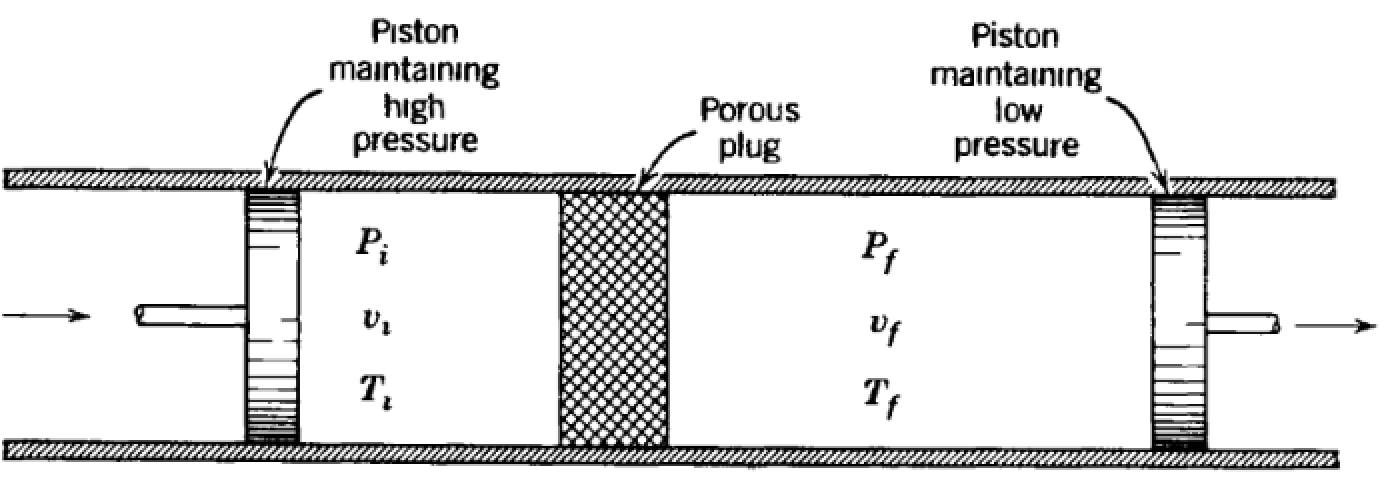
\includegraphics[width = .8\textwidth]{./../Pictures/fig6.2.png}
\caption{Joule-Thomson过程的装置示意图}\label{Fig6.2}
\end{figure}

对于真实气体来说,给定初始和最终压强,温度的改变在某个温度上是正的,在其下是负的。这种从加热到冷却过程的转变温度称为{\it 反转温度};它取决于特定的气体,并且与初始和最终压强有关。为了让节流过程起到冷却气体的作用,它必须先被冷却到转变温度一下。

为了说明Joule-Thomson过程是一个等焓过程,考虑1mole气体通过节流阀。活塞(图\ref{Fig6.2})推动气体做功$P_iv_1$,其中$v_i$是高压侧的气体摩尔体积。% comment: mol到底怎么翻?看校对的意见了
气体从另一侧被压出吼,它对低压$P_f$区的活塞做功$P_fv_f$。通过能量守恒可以得到最后气体的摩尔能量:初始摩尔能量,加上对气体做功$P_iv_i$,减去气体对外做功$P_fv_f$

\begin{figure}[htbp]
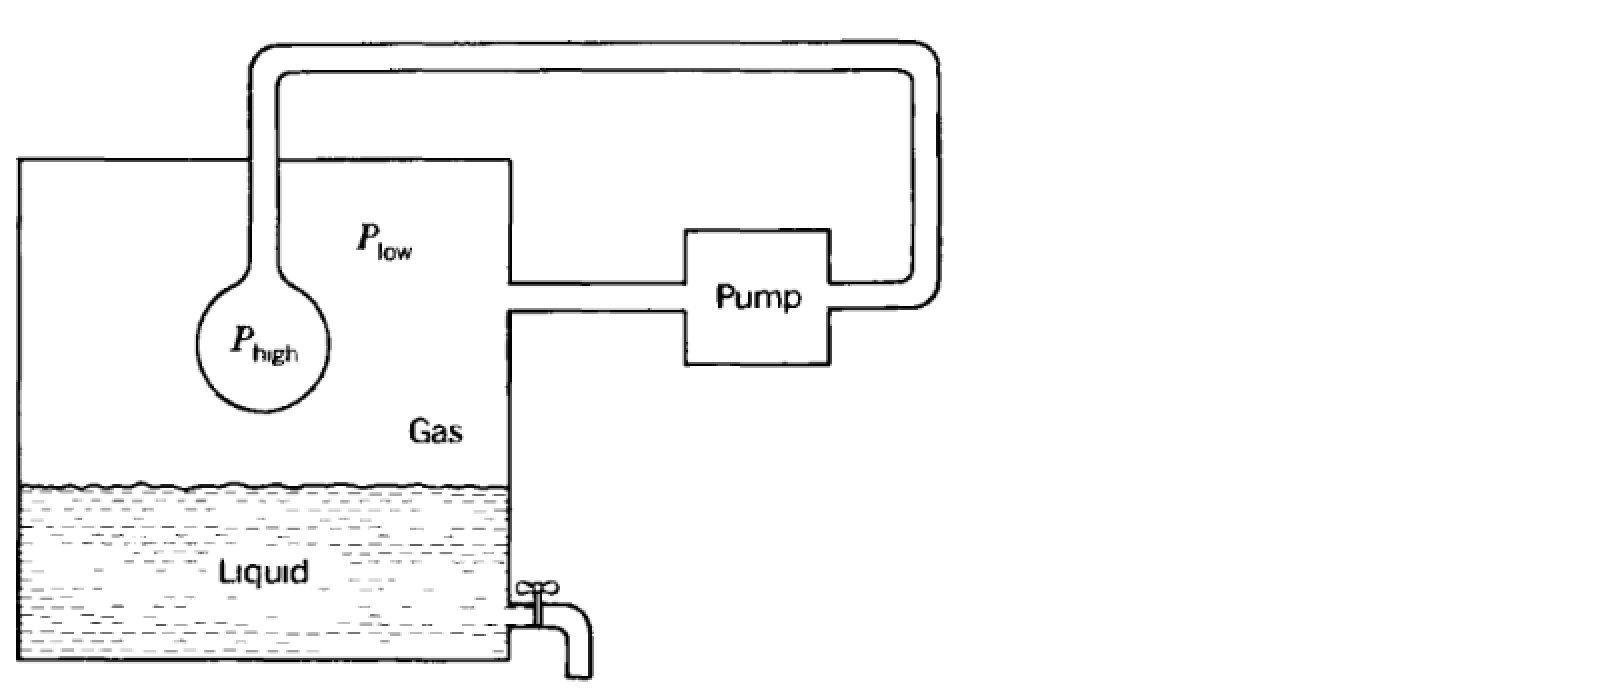
\includegraphics[width = .8\textwidth]{./../Pictures/fig6.3.png}
\caption{节流过程的气体液化装置示意图。泵保持一个恒定气压差($P_{\text{高}}-P_{\text{低}}$)。球形端为高压管,其透过表面的多孔陶瓷层通到节流过程中。}\label{Fig6.3}
\end{figure}

\begin{align}\label{equ6.35}
u_f=u_i+P_iv_i-P_fv_f
\end{align}
或
\begin{align}\label{equ6.36}
u_f+P_fv_f=u_i+P_iv_i
\end{align}
用摩尔焓$h$表示就是
\begin{align}\label{equ6.37}
h_f=h_i
\end{align}

尽管在\eqref{equ6.37}中,我们认为Joule-Thomson过程是一个等焓过程,我们其实只是说明末态的焓等于初态的焓,而对整个过程中发生了什么并不做任何推断;{\it 气体的中间态实际上是非平衡态,其焓也没法定义}。

\begin{figure}[h]
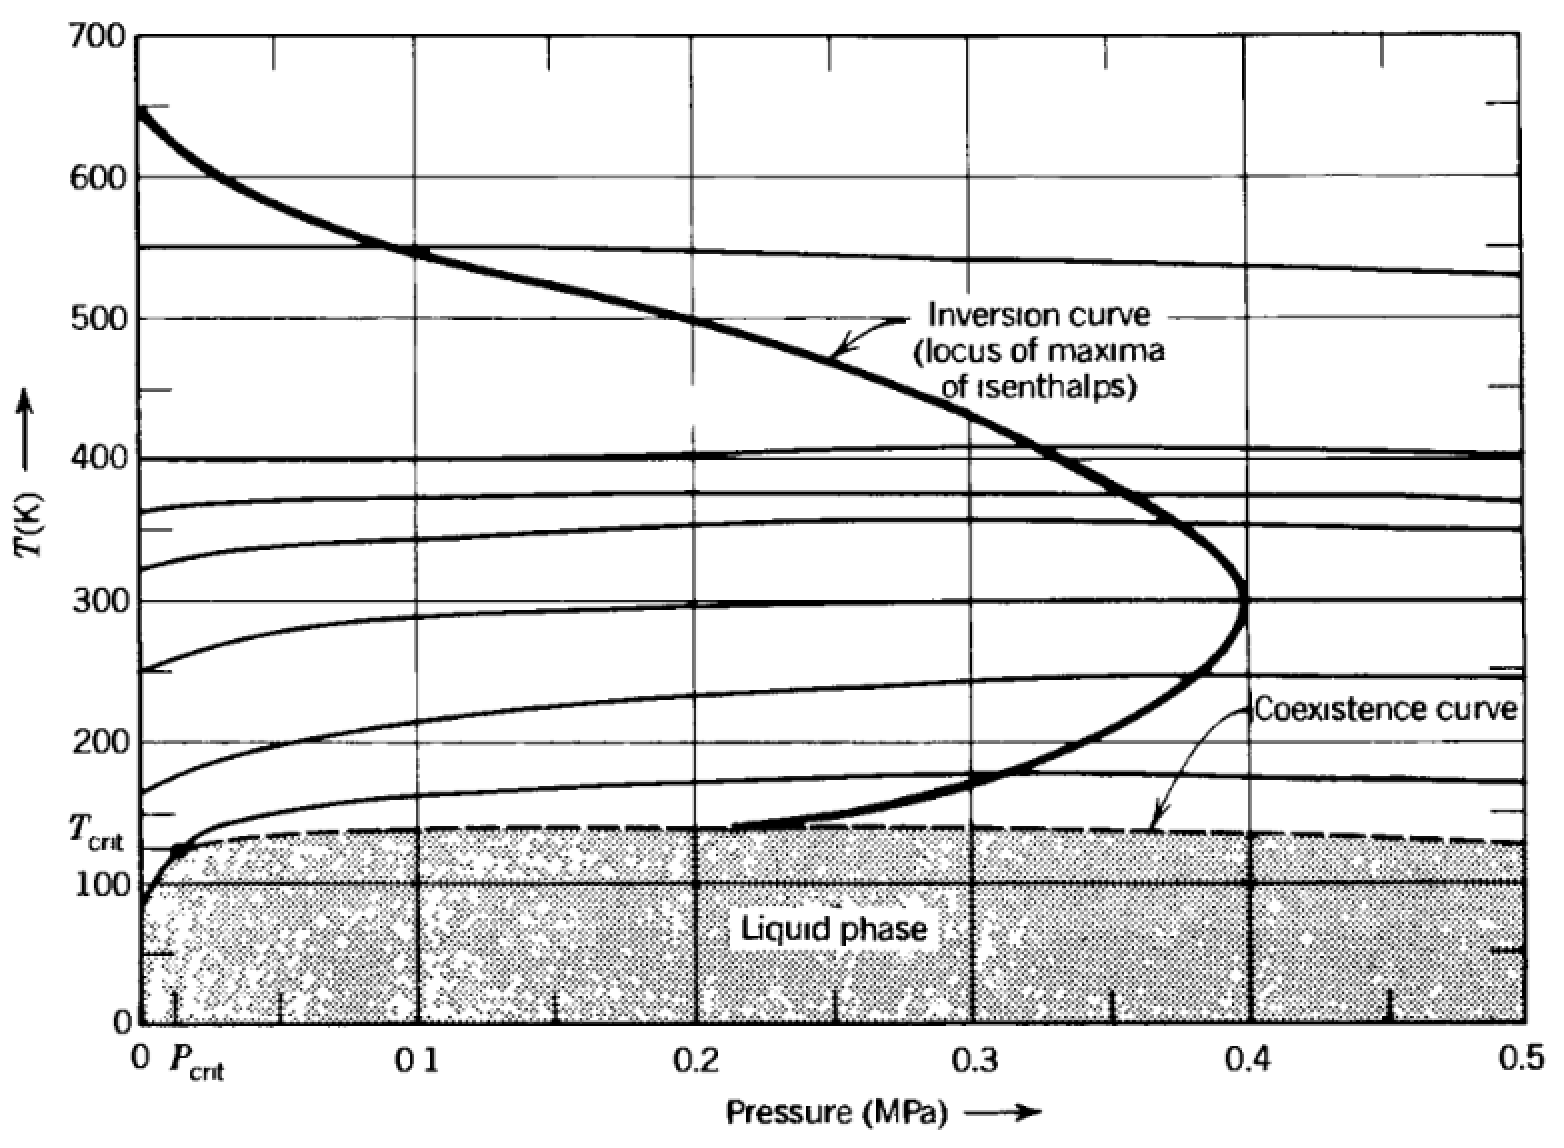
\includegraphics[width = .8\textwidth]{./../Pictures/fig6.4.png}
\caption{氮气的等焓线(实线),温度转换曲线(粗实线),以及气液共存线。半定量的图。}\label{Fig6.4}
\end{figure}

氮气的等焓线如图\ref{Fig6.4}所示,是有顶点的上凸曲线。如果初始温度和压强再这些顶点的左侧,则节流过程将会冷却气体。如果在右侧则压强的微弱减小会加热气体(当然如果有巨大的压强差越过顶点的话就可以冷却或者加热气体)。等焓线的顶点因此就决定了转换曲线,在顶点上小的压强变化不会加热或者冷却气体。%\mpar{此曲线的得出依靠计算Joule-Thomson系数的$0$点连接起来而绘制出来,而Joule-Thomson系数为$\alpha=\left(\dfrac{\partial T}{\partial p}\right)_H$。可以看出转换曲线与等焓线的交点都是等焓线上的斜率为$0$的点。}

图\ref{Fig6.4}的粗实线就是温度转换曲线,吧等焓线的顶点连接起来就行。图中还有气液平衡态的曲线。曲线下的点是液相,上面是气相。共存曲线的端点为``临界点'',在其附近``气体''和``液体''是无法分辨的,其中细节我们在第\ref{chap9}章讲述。

如果节流过程中压强的改变足够小,我们可以用常规的微分来处理
\begin{align}\label{equ6.38}
dT=\left(\frac{\partial T}{\partial P}\right)_{H, N_1, N_2}dP
\end{align}
其可以用标准的测量值($c_P, \alpha, \kappa_T$)的复杂形式表示出来,我们在第\ref{chap7}章会真的写成那种形式。现在呢可以利用数学恒等式\eqref{equA.22}
\begin{align}\label{equ6.39}
dT=-\left[\left(\frac{\partial H}{\partial P}\right)_T/\left(\frac{\partial H}{\partial T}\right)_P\right]dP
\end{align}
其中省略了下标$N_1, N_2,\cdots$,而摩尔数保持不变。然而,$dH=TdS+VdP$是常数,因此
\begin{align}\label{equ6.40}
dT=-\frac{T(\partial S/\partial P)_T+V}{T(\partial S/\partial T)_P}dP
\end{align}
分母部分是$Nc_P$,类比\eqref{equ3.62}或者\eqref{equ3.65}的``Maxwell关系''得到偏微分$(\partial S/\partial P)_T$等于$(-\partial V/\partial T)_P$(在这里利用的是Gibbs势的亮哥交叉导数)。考虑到$(\partial S/\partial P)_T=-(\partial V/\partial T)_P=-V\alpha$(即\eqref{equ3.67})我们终于得到
\begin{align}\label{equ6.41}
dT=\frac{v}{c_P}(T\alpha-1)dP
\end{align}
这是Joule-Thomson效应的基本方程。当压强变化$dP$为负数的时候,$dT$的符号与括号里面的相反。如果$T\alpha>1$,压强的变化(在``节流过程’’中)会冷却气体。反转温度就取决于
\begin{align}\label{equ6.42}
\alpha T_{\text{反转}} = 1
\end{align}

对于理想气体的话热扩散系数$\alpha$等于$1/T$,因此Joule-Thomson过程中没有温度变化。所有的气体在高温和低/中压下都表现的像理想气体,其等焓线变得很``平'',如图\ref{Fig6.4}。真是气体在转变温度上下的升温降温过程我们可以从例子2中看到,并由此来估计转变温度。

\subsection*{例子2}
计算正常的气体的转变温度,假定用van der Waals方程\eqref{equ3.41}来描述
\subsection*{答案}
我们首先必须要计算扩散系数$\alpha$。把van der Waals方程\eqref{equ3.41}对$T$在$P$不变下作微分
\[\alpha = \frac{1}{v}\left(\frac{\partial v}{\partial T}\right)_P=\left[\frac{Tv}{v-b}-\frac{2a(v-b)}{Rv^2}\right]^{-1} \]
把等式右边写成$T$和$P$的函数是不现实的。一个近似的做法是考虑到摩尔体积是在$0.02m^3$这个量级的,因此$b/v$的量级为$10^{-3}$而$a/RTv$则在$10^{-3}-10^{-4}$量级(见表3.1)。因此只保留最低级数的$b/v$和$a/RTv$就可以了。令
\[\epsilon_1\equiv\frac{b}{v}\quad \epsilon_2\equiv\frac{a}{RTv} \]
从而
\[\begin{split}
\alpha&=\left[\frac{T}{1-\epsilon_1}-\frac{2T}{v}(v-b)\epsilon_2\right]^{-1}\\
&=\frac{1}{T}\left[\frac{1}{1-\epsilon_1}-2(1-\epsilon_1)\epsilon_2\right]^{-1}
\end{split} \]
而再利用\eqref{equ6.41}
\[dT=\frac{v}{c_P}(T\alpha-1)dP \]
而同时有
\[T_{\text{反转}}\alpha=1 \]
我们从而得到转变温度时
\[[1-\epsilon_1+2\epsilon_2+\cdots]=1 \]
或者说
\[\epsilon_1=2\epsilon_2 \]
反转温度即为
\[T_{\text{反转}}\simeq\frac{2a}{bR} \]
气体在$T_{\text{反转}}$之下则被制冷,之上则被加热。从表3.1中,我们可以计算一些气体的反转温度:$T_{\text{反转}}(\mathrm{H})_2=224$K,$T_{\text{反转}}(\mathrm{Ne})=302$K,$T_{\text{反转}}(\mathrm{N})_2=850$K,$T_{\text{反转}}(\mathrm{O})_2=1020$K,$T_{\text{反转}}(\mathrm{CO})_2=2260$K。经验上来看,反转温度与压强息息相关——在我们这里的计算中那些被忽略的高阶项们。H$_2$的零压反转温度为$204$K,而氖则是$228$K——这与我们的粗犷的计算是符合的相当好的。对于多原子气体就符合的不那么好了,CO$_2$的测量值为$1275$K而我们计算的结果是$2260$K。


